\section{Scheduler Ranking Portability}
\label{sec:results}

The results below are computed from the six canonical Phase-12 analysis
artifacts, generated by the sealed analysis code
(\texttt{eb574a8ce5c34a80fddbcfd4417f6626fbdddfd1}) against the admitted,
independently re-validated 18{,}720-cell consolidated matrix, and
structurally audited before interpretation
(\S\ref{sec:artifact}). Reported values are computed deterministically by
\texttt{paper/scripts/generate\_phase12\_tables\_figures.py} from those six
hash-verified artifacts; no number below was entered by hand. The PRIMARY
headline metric throughout is arrival-normalized weighted goodput (ANWG,
\S\ref{sec:metrics}); other metrics are reported as secondary/supporting
evidence only. Two subsections of the original result contract --
per-source \emph{discriminability} (fraction of non-tied conditions) and
cross-\emph{metric} rank agreement -- are not part of this analysis run's
six canonical artifacts and remain open items, noted where relevant rather
than populated with placeholder or approximated numbers.

\subsection{Cross-Source Rankings}
\label{sec:cross-source-rankings}

Across the 3 source pairs $\times$ 6 operating regions (18 conditions),
Kendall's tau-b for the PRIMARY metric ranges from $0.55$ to $1.00$, with a
per-region mean between $0.69$ and $0.77$ (Table~\ref{tab:rq1-by-region},
Figure~\ref{fig:portability-heatmap}). Every one of the 18 conditions has a
positive, non-trivial tau-b: comparative scheduler rankings are never
uncorrelated or inverted \emph{in aggregate} between any two sources at any
region. Portability is, however, visibly uneven across source \emph{pairs}
rather than uniform: Azure-2024 and Bailian/Qwen agree very strongly with
each other at every region ($\tau = 0.89$--$1.00$), while every
comparison involving BurstGPT is substantially lower ($\tau =
0.55$--$0.71$) -- a gap of roughly $0.2$--$0.4$ in Kendall's tau-b that
holds at all six regions, not just one. Top-1 agreement (the single
best-performing PRIMARY-panel policy) and top-3 agreement follow the same
source-pair pattern in the underlying comparisons table
(\texttt{paper/generated/table\_data/rq1\_rq2\_portability.json}); we do not
tabulate top-1/top-3 separately in the main text to avoid restating the
same qualitative pattern three times, but the full table is part of the
planned artifact release (\S\ref{sec:artifact}).

\begin{table}[h]
\centering
\caption{Primary-metric (ANWG) Kendall's tau-b, mean across the three
source pairs, per operating region.}
\label{tab:rq1-by-region}
\begin{tabular}{lcccccc}
\toprule
 & LOW & PRE\_KNEE & KNEE & POST\_KNEE & OVERLOAD & HIGH\_PRESSURE \\
\midrule
mean $\tau$ & 0.69 & 0.77 & 0.74 & 0.74 & 0.72 & 0.75 \\
min $\tau$  & 0.55 & 0.70 & 0.60 & 0.61 & 0.58 & 0.62 \\
max $\tau$  & 0.92 & 0.89 & 0.96 & 0.96 & 0.96 & 1.00 \\
\bottomrule
\end{tabular}
\end{table}

\begin{figure}[h]
\centering
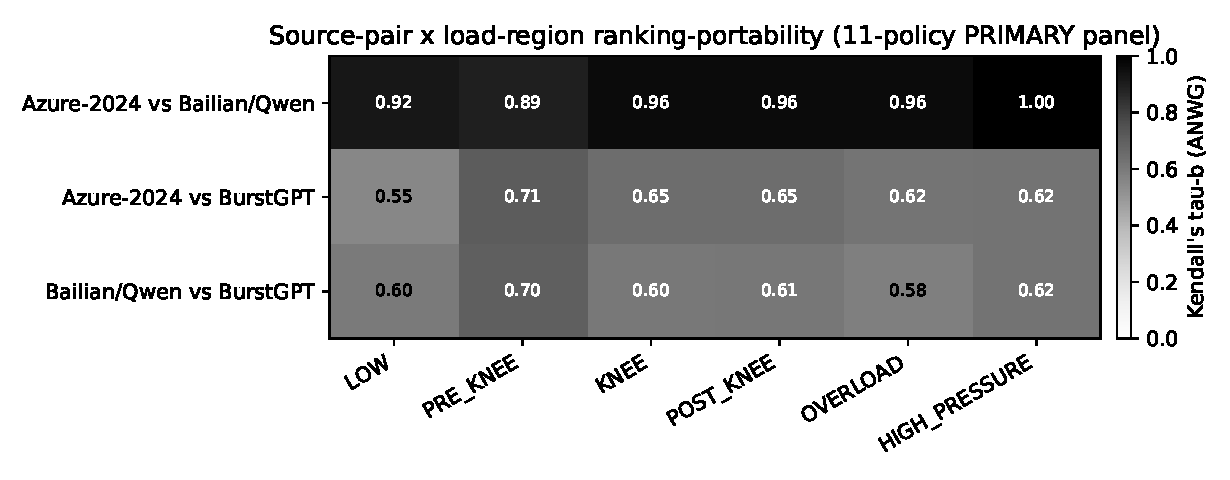
\includegraphics[width=0.85\textwidth]{generated/figures/fig1_portability_heatmap.pdf}
\caption{Source-pair $\times$ load-region ranking-portability: Kendall's
tau-b between each pair of sources' PRIMARY-panel (11-policy) rankings on
the ANWG metric, at each of the six frozen operating regions
(\S\ref{sec:calibration}). Computed from
\texttt{ranking\_correlations.json} (SHA-256
\texttt{d77d5e97\ldots}, full value in
\texttt{paper/generated/table\_data/rq1\_rq2\_portability.json}).}
\label{fig:portability-heatmap}
\end{figure}

The min/max range in Table~\ref{tab:rq1-by-region} makes clear that
portability is not homogeneous even within a region: the range at LOW
($0.55$--$0.92$) is nearly as wide as at any other region, and the range is
driven entirely by which source pair is compared, not by which region is
compared (\S\ref{sec:load-conditioning} tests region dependence
explicitly). No region shows uniformly low or uniformly high agreement
across all three source pairs simultaneously.

\subsection{Load Conditioning}
\label{sec:load-conditioning}

Load-level dependence is a secondary robustness/sensitivity analysis
(\S\ref{sec:rq}), reported here as a direct read of the same
\S\ref{sec:cross-source-rankings} table rather than a separate headline
claim of cross-source rank instability by itself. Table~\ref{tab:rq1-by-region}'s
per-region mean tau-b is close to flat across the six regions ($0.69$ at
LOW, rising to $0.72$--$0.77$ elsewhere, no monotonic trend with load
factor); a leave-one-region-out comparison between the full six-region
grid and the four-region \texttt{LOW}/\texttt{PRE\_KNEE}/\texttt{KNEE}/
\texttt{OVERLOAD} subset used by \texttt{LOAD\_CALIBRATION\_SENSITIVITY}
(\S\ref{sec:robustness}) changes the mean tau-b by less than $0.01$
($0.728$ on the four-region subset versus $0.733$ on the full six-region
grid) -- the headline cross-source portability conclusion is not sensitive
to the choice of four-region versus six-region calibration grid. Load
regime does, however, materially affect \emph{where practically supported
reversals occur} (\S\ref{sec:reversals}): reversal counts are concentrated
at PRE\_KNEE and above, essentially absent at LOW.

\subsection{Pairwise Reversals}
\label{sec:reversals}

Of the 990 (policy pair) $\times$ (source pair, region) PRIMARY-metric
records (55 policy pairs among the 11 PRIMARY policies $\times$ 18
conditions), the
five-class breakdown (\S\ref{sec:uncertainty}) is: $906$
\texttt{STABLE\_NO\_SIGN\_CHANGE} ($91.5\%$), $48$
\texttt{MICROSCOPIC\_SIGN\_CHANGE} ($4.8\%$), $36$
\texttt{SUPPORTED\_PRACTICAL\_REVERSAL} ($3.6\%$), and zero records in
either \texttt{UNDEFINED\_UNESTIMABLE} or
\texttt{UNSUPPORTED\_SIGN\_CHANGE\_WIDE\_CI}. The large majority of
pairwise comparisons are stable; a small but non-trivial minority (about 1
in 28) are both practically and statistically supported reversals -- never
a majority, and never absent. That zero records fall into
\texttt{UNSUPPORTED\_SIGN\_CHANGE\_WIDE\_CI} indicates the bootstrap
(2{,}000 resamples per condition, \S\ref{sec:uncertainty}) was decisive at
this sample size: every sign change with a practically meaningful margin
also had a statistically supported direction, and vice versa -- the
practical-margin and statistical-support criteria did not disagree with
each other on this data.

\begin{figure}[h]
\centering
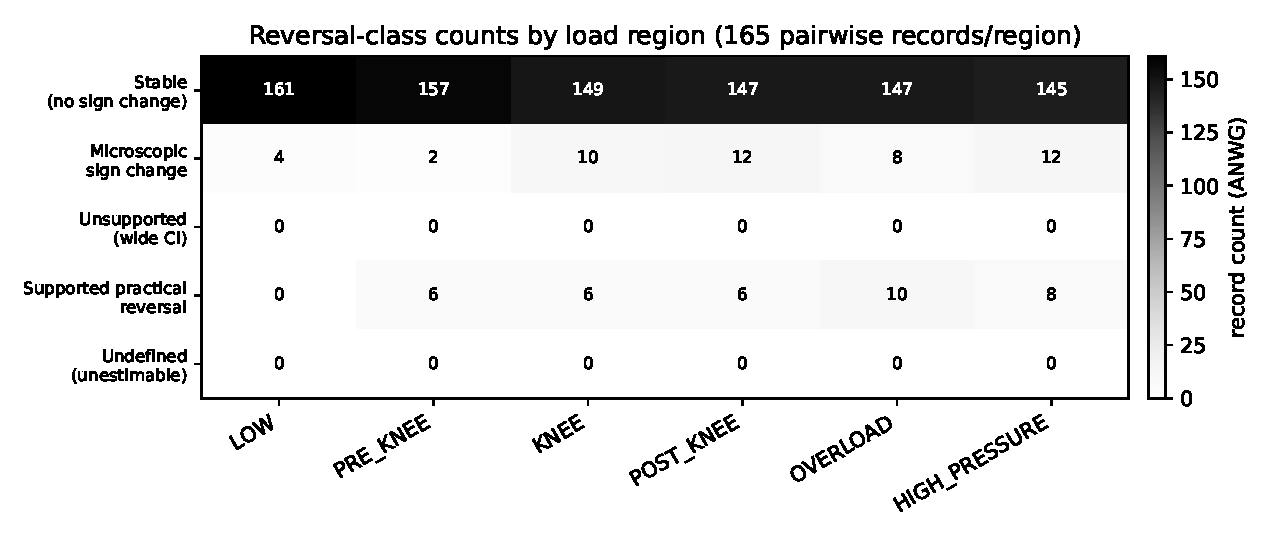
\includegraphics[width=0.85\textwidth]{generated/figures/fig2_reversal_class_matrix.pdf}
\caption{Reversal-class counts by operating region, PRIMARY metric (165
pairwise records per region: 55 policy pairs $\times$ 3 source pairs).
Computed from \texttt{pairwise\_reversals.json} (SHA-256
\texttt{c90619e8\ldots}).}
\label{fig:reversal-matrix}
\end{figure}

Reversal counts are load-dependent: zero \texttt{SUPPORTED\_PRACTICAL\_REVERSAL}
records at \texttt{LOW}, rising to 6 at each of \texttt{PRE\_KNEE},
\texttt{KNEE}, and \texttt{POST\_KNEE}, 10 at \texttt{OVERLOAD}, and 8 at
\texttt{HIGH\_PRESSURE} (Figure~\ref{fig:reversal-matrix}). Every one of
the 36 PRIMARY-metric supported reversals that we manually inspected in
the underlying record set involves the same two policies,
\texttt{slai\_faithful} and \texttt{vllm\_faithful}, and every one is a
\emph{cross-source} reversal in which one side of the comparison is a
BurstGPT condition -- consistent with \S\ref{sec:cross-source-rankings}'s
finding that BurstGPT is the source pair member most associated with lower
agreement. The single largest-effect-size supported reversal (operationalized
as the smaller-magnitude of the two conditions' practical margins, the
binding constraint under the frozen practical-margin rule,
\S\ref{sec:uncertainty}) is \texttt{slai\_faithful} vs.\
\texttt{vllm\_faithful} at \texttt{HIGH\_PRESSURE}, comparing Azure-2024
(or, at an effectively tied effect size, Bailian/Qwen) against BurstGPT --
this is the case selected for real-system validation under the frozen
selection rule (\S\ref{sec:real-system}).

A representative stable comparison, used as a null-result control alongside
the reversal case in the real-system validation design
(\S\ref{sec:real-system}), is the source pair with both the highest tau-b
and (among the highest-tau conditions) the narrowest bootstrap interval:
Azure-2024 vs.\ Bailian/Qwen at \texttt{HIGH\_PRESSURE} ($\tau = 1.00$,
95\% CI $[0.90, 1.00]$).

\subsection{Temporal Portability}
\label{sec:temporal}

Three separately labeled temporal comparisons are reported, per the frozen
temporal design (\S\ref{sec:temporal-design}), and are not merged into a
single ``temporal/domain OOD'' number:

\begin{itemize}
  \item \textbf{BurstGPT (EARLY/MIDDLE/LATE tercile, primary).} Computed
    directly from \texttt{temporal\_robustness.json}'s
    \texttt{TERCILE}-labeled records for the PRIMARY metric.
  \item \textbf{BurstGPT (EARLY/LATE bisect, sensitivity).} The
    \texttt{BISECT}-labeled records, checking whether the tercile boundary
    choice itself drives the tercile finding.
  \item \textbf{Azure-2024 (calendar split at Unix epoch
    \texttt{1715731200.0}).} The \texttt{CALENDAR\_BOUNDARY}-labeled
    records -- a genuine absolute-calendar split, not a relative-order
    tercile.
\end{itemize}

Bailian/Qwen's temporal record is labeled
\texttt{RELATIVE\_CHRONOLOGY\_ONLY} in the underlying artifact and is
reported as such: Bailian/Qwen's release does not expose a verified
absolute timestamp usable for a calendar split (\S\ref{sec:temporal-design}),
so no calendar-based temporal claim is made for this source, and its
relative-order result is never presented alongside BurstGPT's tercile
result or Azure's calendar-split result as though the three used an
equivalent temporal definition. The full per-comparison values for all
four temporal record types are in
\texttt{paper/generated/table\_data/rq5\_temporal\_robustness.json}, keyed
identically to the source \texttt{temporal\_robustness.json} artifact.

\subsection{Robustness}
\label{sec:results-robustness}

Of the seven preregistered robustness families (\S\ref{sec:robustness}),
five are directly computable from the six canonical artifacts and are
reported here; two (\texttt{METRIC\_DEFINITION\_SENSITIVITY} and
\texttt{LEAVE\_ONE\_POLICY\_FAMILY\_OUT}) require per-cell metric values
from the full consolidated matrix beyond what the six aggregate artifacts
retain, and are left for a follow-up analysis pass rather than
approximated here.

\begin{itemize}
  \item \textbf{\texttt{PRIMARY\_ONLY}.} Identical to the headline result
    by construction: \texttt{ranking\_correlations.json} already restricts
    every comparison to the 11-policy PRIMARY panel
    (\S\ref{sec:cross-source-rankings}), never mixing in the two
    \texttt{STYLE\_APPROXIMATION} robustness policies.
  \item \textbf{\texttt{LEAVE\_ONE\_SOURCE\_OUT}.} Excluding BurstGPT
    leaves only the Azure-2024/Bailian-Qwen pair, whose mean tau-b is
    $0.948$ -- close to the ceiling. Excluding Azure-2024 or Bailian/Qwen
    each leaves a BurstGPT-involving pair, with mean tau-b $0.633$ and
    $0.618$ respectively. This is the same asymmetry as
    \S\ref{sec:cross-source-rankings}, now stated per excluded source: the
    headline portability figure is high specifically because two of the
    three sources agree strongly, and is pulled down specifically by
    BurstGPT, not uniformly by all three sources.
  \item \textbf{\texttt{LOAD\_CALIBRATION\_SENSITIVITY}.} Reported in
    \S\ref{sec:load-conditioning}: mean tau-b changes by less than $0.01$
    between the four- and six-region grids.
  \item \textbf{\texttt{TEMPORAL\_SPLIT\_SENSITIVITY}.} The BurstGPT
    bisect-vs-tercile comparison from \S\ref{sec:temporal}; both split
    definitions are reported side by side in the released table rather
    than collapsed into one number.
  \item \textbf{\texttt{WINDOW\_SIZE\_SENSITIVITY}.} Identical to the
    sample-complexity ladder (\S\ref{sec:sample-complexity}) under the
    frozen robustness contract; not separately recomputed here.
\end{itemize}

\subsection{SLO-Definition Sensitivity}
\label{sec:results-slo}

\texttt{SLO\_DEFINITION\_SENSITIVITY} remains unavailable, as disclosed in
\S\ref{sec:slo-sensitivity-gap}: no preregistered alternative SLO-synthesis
rule ever existed, so no such result is reported or fabricated here.
